\section{GT1: The Energy Readout Is Not Closed}
\label{sec:gt1}
%% Packet W-03. Ledger rows: GT1, GB2, NEG.gt1_b_parity_control_open.

\subsection{Claim}

In plain terms: for an aging East chain, knowing the microstate tells you substantially more
about the energy a few steps ahead than knowing the present energy does, and it does so by a
certified factor more than at constrained equilibrium. The packaging defect of \S\ref{sec:methods}
is reported alongside as a second ratio. Precisely:

\claimref{GT1}{a0cea276116f05fcbb10844c527aac69d2027c70210a19db4753364d6c54d44e}
On the declared scope (East model, $N=8$, lens $L_{\mathrm{energy}}$, $\tau$ ladder
$[1,2,4,8]$, quench cell $\epsilon: 7/10 \to 1/10$ with waiting time $t_w = 20$), the closure
deficit $\mathrm{CD}_\tau$ of the aging protocol exceeds the constrained-East
stationary-equilibrium baseline at every declared cell by at least the declared margin $3/2$
(achieved minimum ratio $\approx 1.6392$; Table~\ref{tab:gt1-margins}), and the audited
idempotence-defect table exceeds its declared margin $2$ (achieved ratio $289/121$). Grade:
theorem (audited class); evidence type as declared in the artifact: deterministic float64 for the
CD grid and its margin, exact rational for the idempotence-defect ratio and the lumpability
controls. In the framework's filing vocabulary the claim reads: the P5 channel of the standard
thermodynamic packaging is not \texttt{active\_projection} as a closed packaging on this declared
glassy scope; that is, packaging the present energy readout does not yield a closed description.
Anchors: F-III T8, F-I D-IC-01/D-IC-02/T-CL-01, \sbtcite{sbt-paper-b} Def.~3.1.

\begin{longtable}{rrrr}
\caption{GT1 closure deficit vs. constrained-equilibrium baseline (East N=8, L\_energy)}\label{tab:gt1-margins} \\
\toprule
$\tau$ & $CD_\tau$ (glassy) & $CD_\tau$ (equilibrium) & ratio \\
\midrule
\endfirsthead
\toprule
$\tau$ & $CD_\tau$ (glassy) & $CD_\tau$ (equilibrium) & ratio \\
\midrule
\endhead
\bottomrule
\endfoot
1 & 0.033650 & 0.018875 & 1.7828 \\
2 & 0.063730 & 0.036068 & 1.7669 \\
4 & 0.113110 & 0.065575 & 1.7249 \\
8 & 0.177212 & 0.108112 & 1.6392 \\
\textbf{margin} & -- & -- & declared 3/2, achieved 1.6392 \\
\bottomrule
\end{longtable}


\subsection{The control structure, including a corrected expectation}

The controls deserve emphasis because one of them corrected our own design document. The design
called for constrained-East equilibrium to serve as a zero-deficit control, on the intuition that
an equilibrated chain has nothing left to remember. That intuition is \emph{false}, and provably
so. $\mathrm{CD}_\tau = 0$ if and only if the energy readout is $\tau$-lumpable, and
whether it is depends on the kinetic constraint, not on stationarity: in East a spin can
flip only when its left neighbor is up, so the number of spins free to move, and hence the rate
at which the energy can change, depends on \emph{where} the up spins sit, not merely on how many
there are. So the energy
readout of East is not closed even at equilibrium. The shipped certificate therefore uses two
controls with different jobs (Fig.~\ref{fig:gt1-ladder}): the \emph{unconstrained} model, whose
energy readout is lumpable by construction, sits at exact rational $\mathrm{CD} = 0$ (float
residuals at $10^{-17}$, exact lumpability verified symbolically), while constrained-East
equilibrium is an honest \emph{nonzero baseline}. The content of the certificate is that aging
exceeds even that baseline by the declared margin. Equilibrium is not used as a zero control
anywhere.

\claimref{GB2}{847f389464f9196f2315c05e3cef842efa94f201aad26f19b5dc4071e043f081}
Because the aging chain is driven by a temperature schedule, the closure deficit must be defined
relative to the protocol rather than to a single stationary kernel. The machinery for that is the
GB2 demo: finite protocol-relative CD computations (East versus unconstrained, $N=4$, declared
$\epsilon$ grid) with exactness reserved for the lumpability check and float64 windowed
diagnostics labeled as such. GB2 is recognition-grade, a demonstration rather than a certificate,
and the GT1 artifact carries a passing consistency gate for it: in the stationary limit the
protocol-relative deficit reproduces the stationary deficit with residual exactly $0$.

\begin{figure}[htbp]
  \centering
  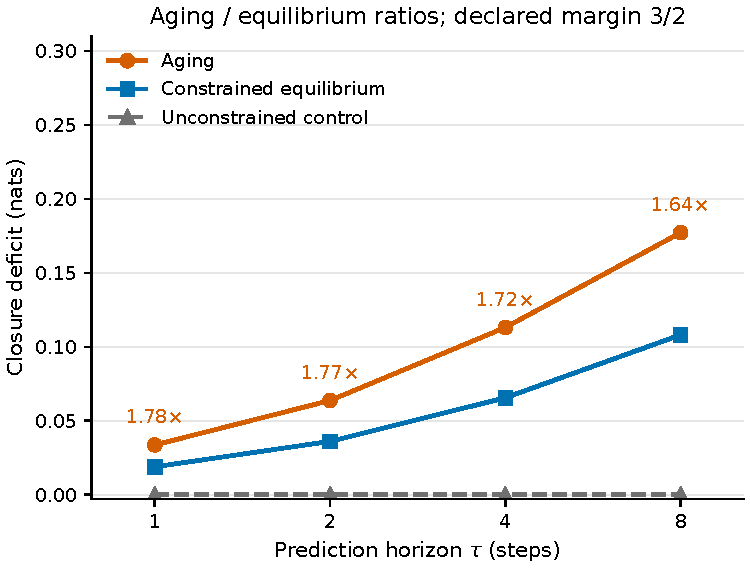
\includegraphics[width=0.7\linewidth]{figures/out/fig_gt1_cd_ladder.pdf}
  \caption{GT1 closure deficit (nats) versus horizon $\tau$: aging protocol, constrained-equilibrium
    baseline (nonzero because the energy readout is not lumpable), and the unconstrained control at
    exact zero. Annotations give the aging/equilibrium ratio at each horizon against the declared
    margin $3/2$.}
  \label{fig:gt1-ladder}
\end{figure}

\subsection{Scope and open control}

The certificate quantifies over exactly its declared cell: East, $N=8$, $L_{\mathrm{energy}}$,
the declared $\tau$ ladder and quench window. FA replication, the richer $L_{\mathrm{panel}}$
lens, and $N=10$ are extensions that were not run, listed as such in the artifact envelope.

\claimref{NEG.gt1\_b\_parity\_control\_open}{a0cea276116f05fcbb10844c527aac69d2027c70210a19db4753364d6c54d44e}
One intended control is open: the paper-[B] example-chain benchmark-parity check was not ported,
and the GT1 artifact files it as an explicitly skipped control with its reason
(machine-readable \texttt{status: skipped}). The certificate's margins are internal to its own
declared scope and do not route through [B]'s example chains; no [B]-parity is claimed until the
control is actually run.
